\documentclass[twoside]{book}

% Packages required by doxygen
\usepackage{fixltx2e}
\usepackage{calc}
\usepackage{doxygen}
\usepackage[export]{adjustbox} % also loads graphicx
\usepackage{graphicx}
\usepackage[utf8]{inputenc}
\usepackage{makeidx}
\usepackage{multicol}
\usepackage{multirow}
\PassOptionsToPackage{warn}{textcomp}
\usepackage{textcomp}
\usepackage[nointegrals]{wasysym}
\usepackage[table]{xcolor}

% Font selection
\usepackage[T1]{fontenc}
\usepackage[scaled=.90]{helvet}
\usepackage{courier}
\usepackage{amssymb}
\usepackage{sectsty}
\renewcommand{\familydefault}{\sfdefault}
\allsectionsfont{%
  \fontseries{bc}\selectfont%
  \color{darkgray}%
}
\renewcommand{\DoxyLabelFont}{%
  \fontseries{bc}\selectfont%
  \color{darkgray}%
}
\newcommand{\+}{\discretionary{\mbox{\scriptsize$\hookleftarrow$}}{}{}}

% Page & text layout
\usepackage{geometry}
\geometry{%
  a4paper,%
  top=2.5cm,%
  bottom=2.5cm,%
  left=2.5cm,%
  right=2.5cm%
}
\tolerance=750
\hfuzz=15pt
\hbadness=750
\setlength{\emergencystretch}{15pt}
\setlength{\parindent}{0cm}
\setlength{\parskip}{0.2cm}
\makeatletter
\renewcommand{\paragraph}{%
  \@startsection{paragraph}{4}{0ex}{-1.0ex}{1.0ex}{%
    \normalfont\normalsize\bfseries\SS@parafont%
  }%
}
\renewcommand{\subparagraph}{%
  \@startsection{subparagraph}{5}{0ex}{-1.0ex}{1.0ex}{%
    \normalfont\normalsize\bfseries\SS@subparafont%
  }%
}
\makeatother

% Headers & footers
\usepackage{fancyhdr}
\pagestyle{fancyplain}
\fancyhead[LE]{\fancyplain{}{\bfseries\thepage}}
\fancyhead[CE]{\fancyplain{}{}}
\fancyhead[RE]{\fancyplain{}{\bfseries\leftmark}}
\fancyhead[LO]{\fancyplain{}{\bfseries\rightmark}}
\fancyhead[CO]{\fancyplain{}{}}
\fancyhead[RO]{\fancyplain{}{\bfseries\thepage}}
\fancyfoot[LE]{\fancyplain{}{}}
\fancyfoot[CE]{\fancyplain{}{}}
\fancyfoot[RE]{\fancyplain{}{\bfseries\scriptsize Generated on Thu Jan 15 2015 15\+:15\+:13 for Police by Doxygen }}
\fancyfoot[LO]{\fancyplain{}{\bfseries\scriptsize Generated on Thu Jan 15 2015 15\+:15\+:13 for Police by Doxygen }}
\fancyfoot[CO]{\fancyplain{}{}}
\fancyfoot[RO]{\fancyplain{}{}}
\renewcommand{\footrulewidth}{0.4pt}
\renewcommand{\chaptermark}[1]{%
  \markboth{#1}{}%
}
\renewcommand{\sectionmark}[1]{%
  \markright{\thesection\ #1}%
}

% Indices & bibliography
\usepackage{natbib}
\usepackage[titles]{tocloft}
\setcounter{tocdepth}{3}
\setcounter{secnumdepth}{5}
\makeindex

% Hyperlinks (required, but should be loaded last)
\usepackage{ifpdf}
\ifpdf
  \usepackage[pdftex,pagebackref=true]{hyperref}
\else
  \usepackage[ps2pdf,pagebackref=true]{hyperref}
\fi
\hypersetup{%
  colorlinks=true,%
  linkcolor=blue,%
  citecolor=blue,%
  unicode%
}

% Custom commands
\newcommand{\clearemptydoublepage}{%
  \newpage{\pagestyle{empty}\cleardoublepage}%
}


%===== C O N T E N T S =====

\begin{document}

% Titlepage & ToC
\hypersetup{pageanchor=false,
             bookmarks=true,
             bookmarksnumbered=true,
             pdfencoding=unicode
            }
\pagenumbering{roman}
\begin{titlepage}
\vspace*{7cm}
\begin{center}%
{\Large Police }\\
\vspace*{1cm}
{\large Generated by Doxygen 1.8.9.1}\\
\vspace*{0.5cm}
{\small Thu Jan 15 2015 15:15:13}\\
\end{center}
\end{titlepage}
\clearemptydoublepage
\tableofcontents
\clearemptydoublepage
\pagenumbering{arabic}
\hypersetup{pageanchor=true}

%--- Begin generated contents ---
\chapter{Hierarchical Index}
\section{Class Hierarchy}
This inheritance list is sorted roughly, but not completely, alphabetically\+:\begin{DoxyCompactList}
\item Mono\+Behaviour\begin{DoxyCompactList}
\item \contentsline{section}{camera\+Drag\+V2}{\pageref{classcamera_drag_v2}}{}
\item \contentsline{section}{camera\+Drag\+V4}{\pageref{classcamera_drag_v4}}{}
\item \contentsline{section}{clicker}{\pageref{classclicker}}{}
\item \contentsline{section}{gui\+Creator}{\pageref{classgui_creator}}{}
\item \contentsline{section}{main\+Menu\+G\+U\+I}{\pageref{classmain_menu_g_u_i}}{}
\item \contentsline{section}{mouse\+Ray\+Hit}{\pageref{classmouse_ray_hit}}{}
\item \contentsline{section}{movement}{\pageref{classmovement}}{}
\item \contentsline{section}{random\+Instance}{\pageref{classrandom_instance}}{}
\item \contentsline{section}{store\+Cars}{\pageref{classstore_cars}}{}
\end{DoxyCompactList}
\end{DoxyCompactList}

\chapter{Class Index}
\section{Class List}
Here are the classes, structs, unions and interfaces with brief descriptions\+:\begin{DoxyCompactList}
\item\contentsline{section}{\hyperlink{classcamera_drag_v2}{camera\+Drag\+V2} }{\pageref{classcamera_drag_v2}}{}
\item\contentsline{section}{\hyperlink{classcamera_drag_v4}{camera\+Drag\+V4} }{\pageref{classcamera_drag_v4}}{}
\item\contentsline{section}{\hyperlink{classclicker}{clicker} }{\pageref{classclicker}}{}
\item\contentsline{section}{\hyperlink{classgui_creator}{gui\+Creator} }{\pageref{classgui_creator}}{}
\item\contentsline{section}{\hyperlink{classmain_menu_g_u_i}{main\+Menu\+G\+U\+I} }{\pageref{classmain_menu_g_u_i}}{}
\item\contentsline{section}{\hyperlink{classmouse_ray_hit}{mouse\+Ray\+Hit} }{\pageref{classmouse_ray_hit}}{}
\item\contentsline{section}{\hyperlink{classmovement}{movement} }{\pageref{classmovement}}{}
\item\contentsline{section}{\hyperlink{classrandom_instance}{random\+Instance} }{\pageref{classrandom_instance}}{}
\item\contentsline{section}{\hyperlink{classstore_cars}{store\+Cars} }{\pageref{classstore_cars}}{}
\end{DoxyCompactList}

\chapter{Class Documentation}
\hypertarget{classcamera_drag_v2}{}\section{camera\+Drag\+V2 Class Reference}
\label{classcamera_drag_v2}\index{camera\+Drag\+V2@{camera\+Drag\+V2}}
Inheritance diagram for camera\+Drag\+V2\+:\begin{figure}[H]
\begin{center}
\leavevmode
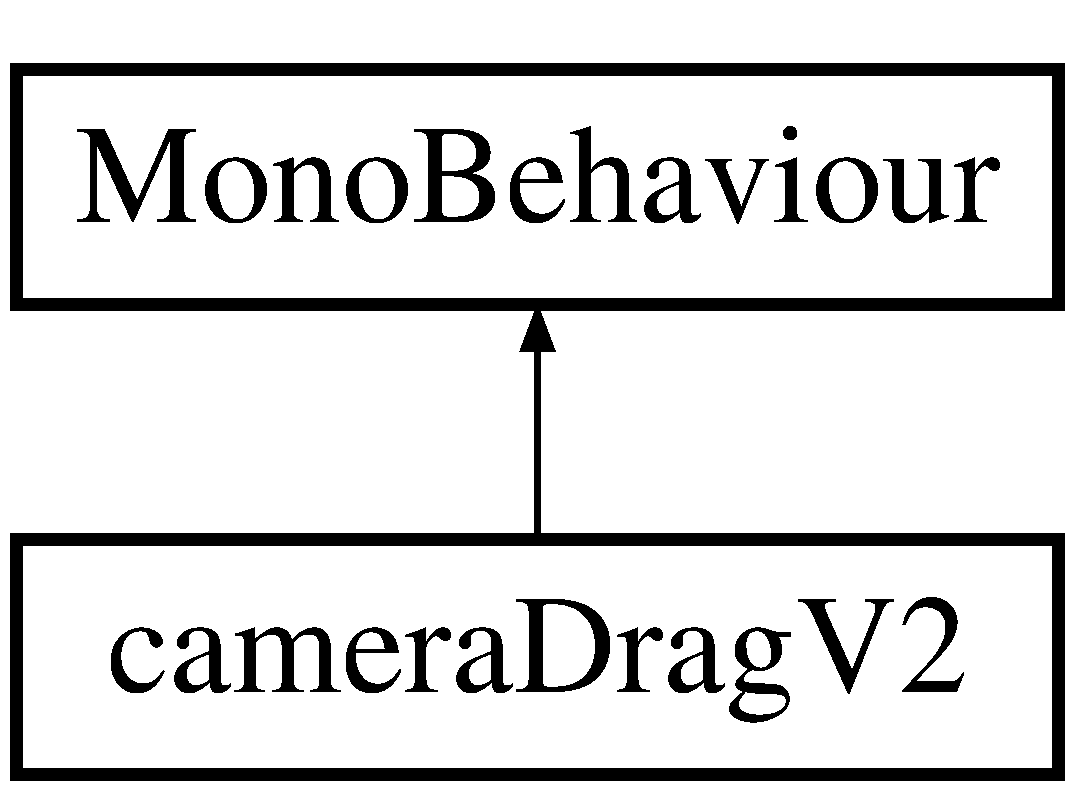
\includegraphics[height=2.000000cm]{classcamera_drag_v2}
\end{center}
\end{figure}
\subsection*{Public Attributes}
\begin{DoxyCompactItemize}
\item 
\hypertarget{classcamera_drag_v2_aa63d90bcfd0e4fa348855460560fc8fd}{}float {\bfseries drag\+Speed}\label{classcamera_drag_v2_aa63d90bcfd0e4fa348855460560fc8fd}

\item 
\hypertarget{classcamera_drag_v2_a9007ac93c7cde56d8479104c9f4c1f5d}{}int {\bfseries min\+X}\label{classcamera_drag_v2_a9007ac93c7cde56d8479104c9f4c1f5d}

\item 
\hypertarget{classcamera_drag_v2_a86d90a914fece47ed346eada75a65373}{}int {\bfseries max\+X}\label{classcamera_drag_v2_a86d90a914fece47ed346eada75a65373}

\item 
\hypertarget{classcamera_drag_v2_a923a09f1df1dc349b5edfb92ecf775d4}{}int {\bfseries min\+Z}\label{classcamera_drag_v2_a923a09f1df1dc349b5edfb92ecf775d4}

\item 
\hypertarget{classcamera_drag_v2_a7fb0fd25618ed259c3340bc953fcc96b}{}int {\bfseries max\+Z}\label{classcamera_drag_v2_a7fb0fd25618ed259c3340bc953fcc96b}

\item 
\hypertarget{classcamera_drag_v2_ac10694452821d5120cae9981ec8058cd}{}int {\bfseries top\+Margin}\label{classcamera_drag_v2_ac10694452821d5120cae9981ec8058cd}

\item 
\hypertarget{classcamera_drag_v2_aed6ee912be0ae6789cedb03e6244c1ed}{}int {\bfseries zoom\+Max\+Size}\label{classcamera_drag_v2_aed6ee912be0ae6789cedb03e6244c1ed}

\item 
\hypertarget{classcamera_drag_v2_a2f6741d854354d83f88cd0ec6a2b6bab}{}int {\bfseries zoom\+Min\+Size}\label{classcamera_drag_v2_a2f6741d854354d83f88cd0ec6a2b6bab}

\end{DoxyCompactItemize}


The documentation for this class was generated from the following file\+:\begin{DoxyCompactItemize}
\item 
Assets/\+\_\+\+Scripts/camera\+Drag\+V2.\+cs\end{DoxyCompactItemize}

\hypertarget{classcamera_drag_v4}{}\section{camera\+Drag\+V4 Class Reference}
\label{classcamera_drag_v4}\index{camera\+Drag\+V4@{camera\+Drag\+V4}}
Inheritance diagram for camera\+Drag\+V4\+:\begin{figure}[H]
\begin{center}
\leavevmode
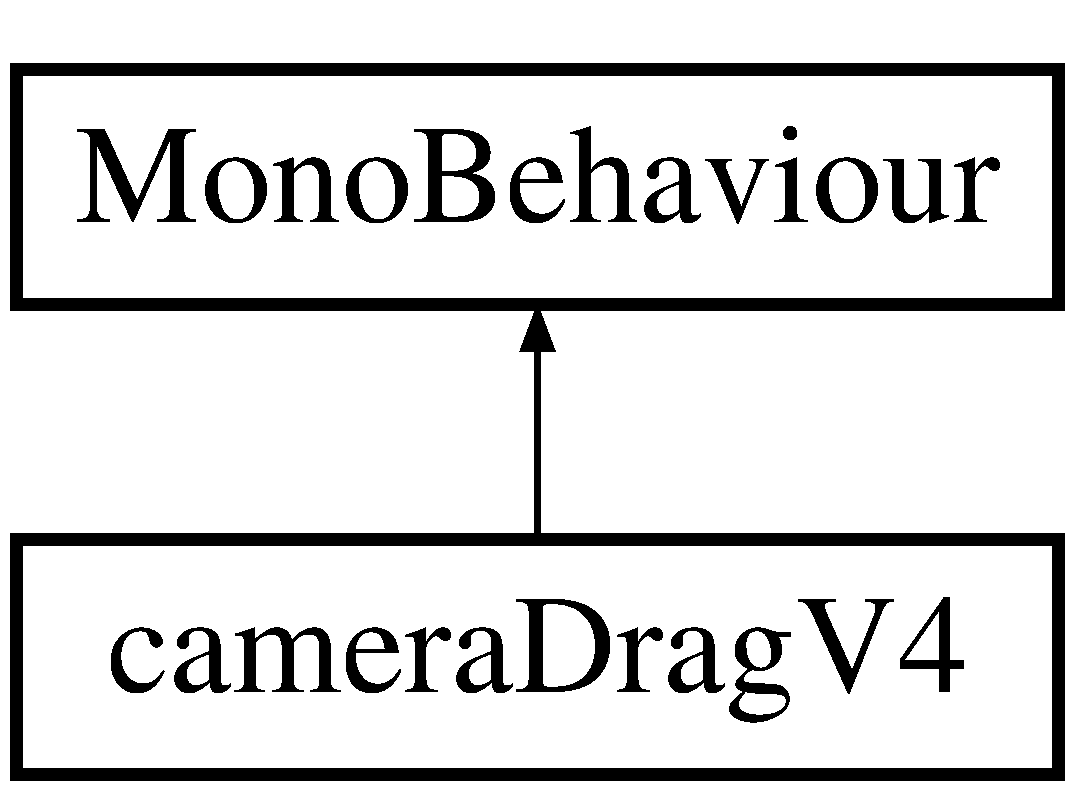
\includegraphics[height=2.000000cm]{classcamera_drag_v4}
\end{center}
\end{figure}
\subsection*{Public Attributes}
\begin{DoxyCompactItemize}
\item 
\hypertarget{classcamera_drag_v4_a80f8856241afcd5c2f165eaf5c40929f}{}int {\bfseries zoom\+Max\+Size}\label{classcamera_drag_v4_a80f8856241afcd5c2f165eaf5c40929f}

\item 
\hypertarget{classcamera_drag_v4_a82e328f5ca7388c79bd4ac16ef284a8c}{}int {\bfseries zoom\+Min\+Size}\label{classcamera_drag_v4_a82e328f5ca7388c79bd4ac16ef284a8c}

\item 
\hypertarget{classcamera_drag_v4_a514fb1fd0d0e31048c91dac30029cb8f}{}int {\bfseries min\+X}\label{classcamera_drag_v4_a514fb1fd0d0e31048c91dac30029cb8f}

\item 
\hypertarget{classcamera_drag_v4_aaadeccba5dd760e761724fe92ca99f6c}{}int {\bfseries max\+X}\label{classcamera_drag_v4_aaadeccba5dd760e761724fe92ca99f6c}

\item 
\hypertarget{classcamera_drag_v4_a164102ae02bf95a3f6250f0fcc2393f2}{}int {\bfseries min\+Z}\label{classcamera_drag_v4_a164102ae02bf95a3f6250f0fcc2393f2}

\item 
\hypertarget{classcamera_drag_v4_a09d6958647698f6d211b696ce21e865b}{}int {\bfseries max\+Z}\label{classcamera_drag_v4_a09d6958647698f6d211b696ce21e865b}

\item 
\hypertarget{classcamera_drag_v4_a0f75833bc85122ab7a88f7e443842090}{}int {\bfseries scroll\+Distance} = 5\label{classcamera_drag_v4_a0f75833bc85122ab7a88f7e443842090}

\item 
\hypertarget{classcamera_drag_v4_a8af87ef0c3dde602cc6c4e70546209db}{}int {\bfseries scroll\+Speed} = 70\label{classcamera_drag_v4_a8af87ef0c3dde602cc6c4e70546209db}

\item 
\hypertarget{classcamera_drag_v4_a091bce69104ddbf27fbb896b7188cdbc}{}int {\bfseries scroll\+Scaling\+Speed}\label{classcamera_drag_v4_a091bce69104ddbf27fbb896b7188cdbc}

\end{DoxyCompactItemize}


The documentation for this class was generated from the following file\+:\begin{DoxyCompactItemize}
\item 
Assets/\+\_\+\+Scripts/camera\+Drag\+V4.\+cs\end{DoxyCompactItemize}

\hypertarget{classclicker}{}\section{clicker Class Reference}
\label{classclicker}\index{clicker@{clicker}}
Inheritance diagram for clicker\+:\begin{figure}[H]
\begin{center}
\leavevmode
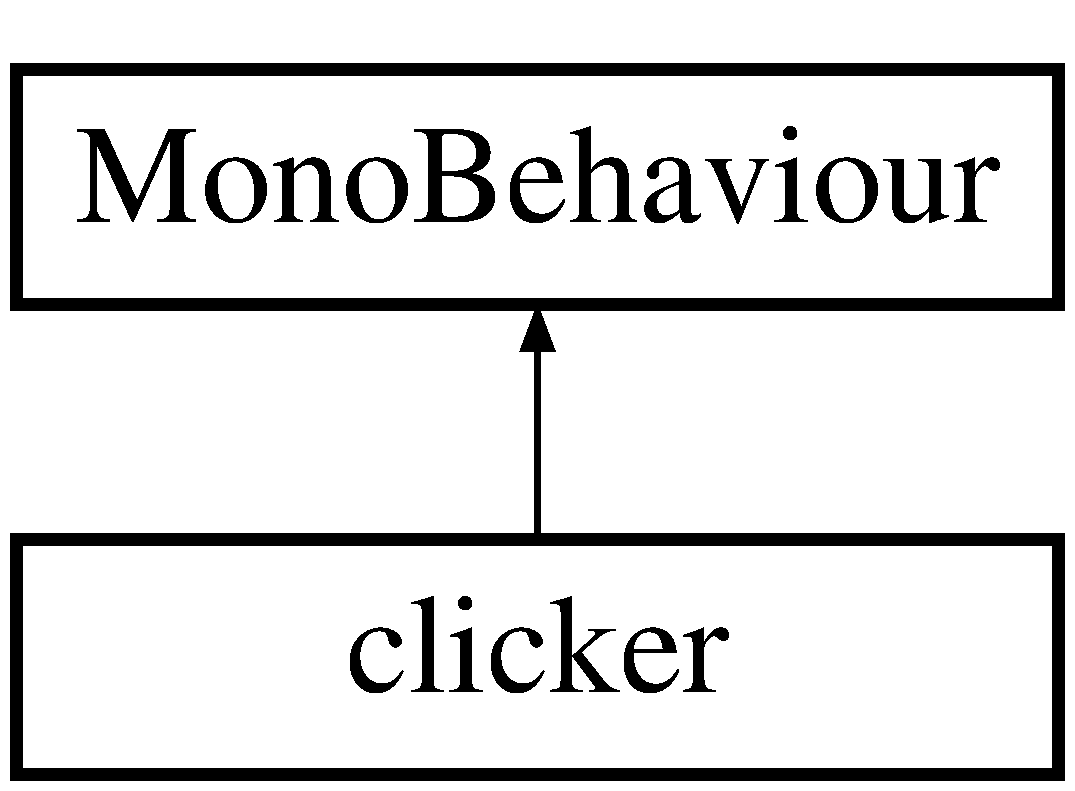
\includegraphics[height=2.000000cm]{classclicker}
\end{center}
\end{figure}
\subsection*{Public Attributes}
\begin{DoxyCompactItemize}
\item 
\hypertarget{classclicker_a22e9b7046b7f47f3bbcb928615f833b6}{}Game\+Object {\bfseries police\+Car}\label{classclicker_a22e9b7046b7f47f3bbcb928615f833b6}

\item 
\hypertarget{classclicker_a13451e7e1c0c4920c7f5a1ecf8f016ee}{}Transform {\bfseries target}\label{classclicker_a13451e7e1c0c4920c7f5a1ecf8f016ee}

\item 
\hypertarget{classclicker_a338a906d61a23e315a4d073faf9e1de9}{}Game\+Object {\bfseries garage}\label{classclicker_a338a906d61a23e315a4d073faf9e1de9}

\end{DoxyCompactItemize}
\subsection*{Static Public Attributes}
\begin{DoxyCompactItemize}
\item 
\hypertarget{classclicker_a83c717841ba9faef75c0ca80671e6b03}{}static int {\bfseries crime\+Clicked} = 0\label{classclicker_a83c717841ba9faef75c0ca80671e6b03}

\item 
\hypertarget{classclicker_a47bc3c4c4fe624aec1d6726433282fa0}{}static int {\bfseries success\+Chance\+G\+U\+I}\label{classclicker_a47bc3c4c4fe624aec1d6726433282fa0}

\end{DoxyCompactItemize}


The documentation for this class was generated from the following file\+:\begin{DoxyCompactItemize}
\item 
Assets/\+\_\+\+Scripts/clicker.\+cs\end{DoxyCompactItemize}

\hypertarget{classgui_creator}{}\section{gui\+Creator Class Reference}
\label{classgui_creator}\index{gui\+Creator@{gui\+Creator}}
Inheritance diagram for gui\+Creator\+:\begin{figure}[H]
\begin{center}
\leavevmode
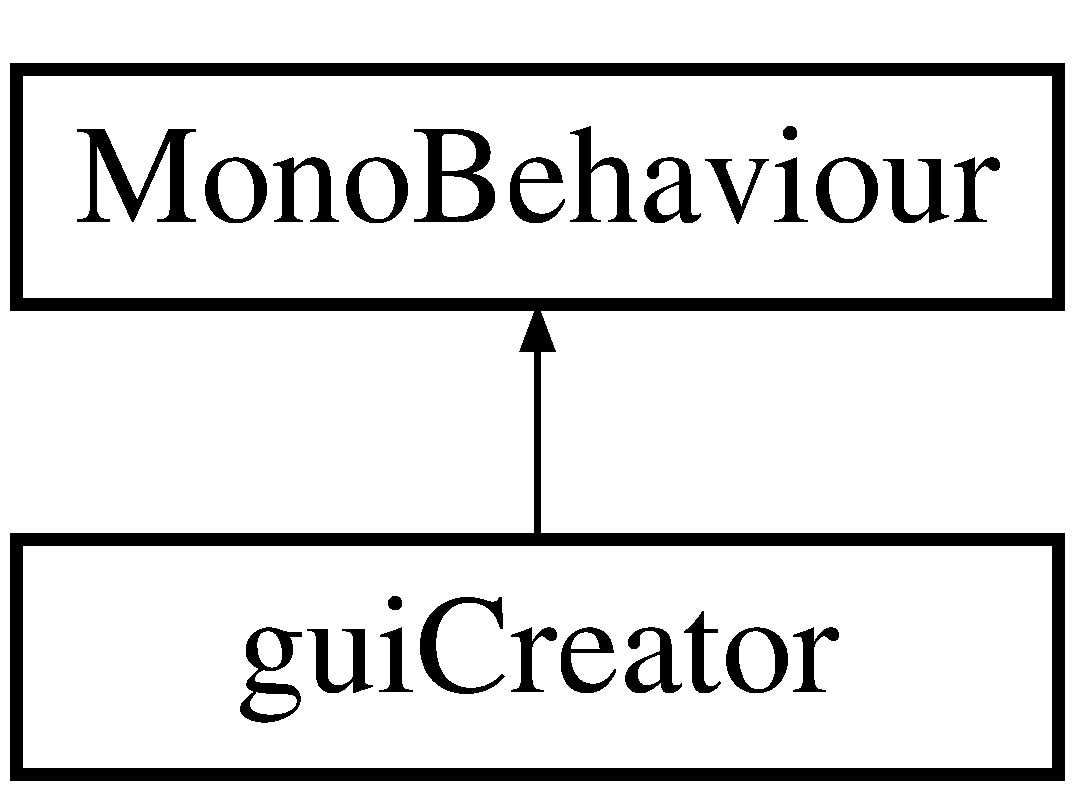
\includegraphics[height=2.000000cm]{classgui_creator}
\end{center}
\end{figure}
\subsection*{Public Attributes}
\begin{DoxyCompactItemize}
\item 
\hypertarget{classgui_creator_a915a23fd9f336553844713a639ad83e3}{}int {\bfseries x\+Test\+Start}\label{classgui_creator_a915a23fd9f336553844713a639ad83e3}

\item 
\hypertarget{classgui_creator_a70c598853d1812c600a4146210344806}{}int {\bfseries y\+Test\+Start}\label{classgui_creator_a70c598853d1812c600a4146210344806}

\item 
\hypertarget{classgui_creator_a690768f5c2091838f1b41966382dc594}{}int {\bfseries x\+Test\+Finish}\label{classgui_creator_a690768f5c2091838f1b41966382dc594}

\item 
\hypertarget{classgui_creator_a471bce16fc0873f6ac6b540aa1703f9f}{}int {\bfseries y\+Test\+Finish}\label{classgui_creator_a471bce16fc0873f6ac6b540aa1703f9f}

\item 
\hypertarget{classgui_creator_adef0435d08f3f6c6ac4cebf713c7fd12}{}Texture {\bfseries background}\label{classgui_creator_adef0435d08f3f6c6ac4cebf713c7fd12}

\item 
\hypertarget{classgui_creator_ab500f649e7b9d10523581ed661fa151e}{}Texture {\bfseries menu\+Background}\label{classgui_creator_ab500f649e7b9d10523581ed661fa151e}

\item 
\hypertarget{classgui_creator_a61327140d7b1374eab045ebc12f04310}{}Texture {\bfseries unit}\label{classgui_creator_a61327140d7b1374eab045ebc12f04310}

\item 
\hypertarget{classgui_creator_a67988a597f26c269830b31a843a0b39b}{}Texture {\bfseries money}\label{classgui_creator_a67988a597f26c269830b31a843a0b39b}

\item 
\hypertarget{classgui_creator_a732384ffcf0f98fdebf766007159d8fc}{}Texture {\bfseries unit\+Symbol}\label{classgui_creator_a732384ffcf0f98fdebf766007159d8fc}

\item 
\hypertarget{classgui_creator_ab5fe099998eb10edc9fd1466218c7c8d}{}G\+U\+I\+Skin {\bfseries tool\+Bar\+Skin}\label{classgui_creator_ab5fe099998eb10edc9fd1466218c7c8d}

\item 
\hypertarget{classgui_creator_a78fbf9a3780f8cb63f2cd51b69a2066f}{}G\+U\+I\+Skin {\bfseries plus\+Skin}\label{classgui_creator_a78fbf9a3780f8cb63f2cd51b69a2066f}

\item 
\hypertarget{classgui_creator_a481736f784475beaa5253628c6ab46cb}{}G\+U\+I\+Skin {\bfseries minus\+Skin}\label{classgui_creator_a481736f784475beaa5253628c6ab46cb}

\item 
\hypertarget{classgui_creator_a66452bd1954665f294a0127383efd2f7}{}G\+U\+I\+Skin {\bfseries done\+Skin}\label{classgui_creator_a66452bd1954665f294a0127383efd2f7}

\item 
\hypertarget{classgui_creator_adf1c870dacc5cc4bbab00d4f274deeee}{}G\+U\+I\+Skin {\bfseries storage\+Skin}\label{classgui_creator_adf1c870dacc5cc4bbab00d4f274deeee}

\item 
\hypertarget{classgui_creator_a2226e699ec3bf91ea80b210c9376140c}{}G\+U\+I\+Skin {\bfseries time\+Skin}\label{classgui_creator_a2226e699ec3bf91ea80b210c9376140c}

\item 
\hypertarget{classgui_creator_af6220451788414eec55bd81f7748db5c}{}G\+U\+I\+Skin {\bfseries pause\+Skin}\label{classgui_creator_af6220451788414eec55bd81f7748db5c}

\item 
\hypertarget{classgui_creator_a75a5f451568ba891e05490969102a1bf}{}G\+U\+I\+Skin {\bfseries play\+Skin}\label{classgui_creator_a75a5f451568ba891e05490969102a1bf}

\item 
\hypertarget{classgui_creator_ae1c4f2d8d26b7ad3080704a21bb4e56d}{}G\+U\+I\+Skin {\bfseries fast\+Skin}\label{classgui_creator_ae1c4f2d8d26b7ad3080704a21bb4e56d}

\item 
\hypertarget{classgui_creator_af3d3c0f591a6a8132af9866f8014c706}{}G\+U\+I\+Skin {\bfseries unit\+Skin}\label{classgui_creator_af3d3c0f591a6a8132af9866f8014c706}

\item 
\hypertarget{classgui_creator_abd680321d06149af3a68b2e51ac953f1}{}G\+U\+I\+Skin {\bfseries menu\+Label\+Skin}\label{classgui_creator_abd680321d06149af3a68b2e51ac953f1}

\end{DoxyCompactItemize}
\subsection*{Static Public Attributes}
\begin{DoxyCompactItemize}
\item 
\hypertarget{classgui_creator_ad3bf7aa843b0a0304c98ebd2d2b61fd2}{}static int {\bfseries done\+Clicked} = 0\label{classgui_creator_ad3bf7aa843b0a0304c98ebd2d2b61fd2}

\item 
\hypertarget{classgui_creator_a333c8fa8c7e68fcfb6d903333180517a}{}static bool {\bfseries pause\+Clicked} = false\label{classgui_creator_a333c8fa8c7e68fcfb6d903333180517a}

\end{DoxyCompactItemize}


The documentation for this class was generated from the following file\+:\begin{DoxyCompactItemize}
\item 
Assets/\+\_\+\+Scripts/gui\+Creator.\+cs\end{DoxyCompactItemize}

\hypertarget{classmain_menu_g_u_i}{}\section{main\+Menu\+G\+U\+I Class Reference}
\label{classmain_menu_g_u_i}\index{main\+Menu\+G\+U\+I@{main\+Menu\+G\+U\+I}}
Inheritance diagram for main\+Menu\+G\+U\+I\+:\begin{figure}[H]
\begin{center}
\leavevmode
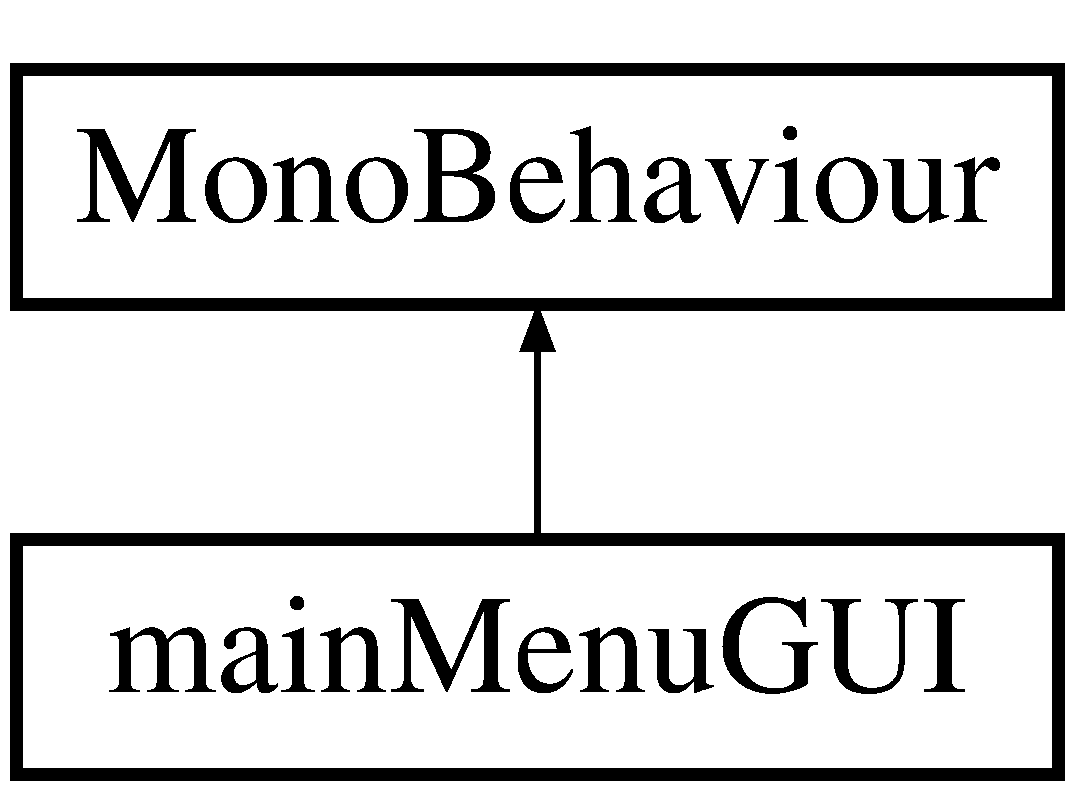
\includegraphics[height=2.000000cm]{classmain_menu_g_u_i}
\end{center}
\end{figure}
\subsection*{Public Attributes}
\begin{DoxyCompactItemize}
\item 
\hypertarget{classmain_menu_g_u_i_a42b7f36725e4c2015762aaeecf74533c}{}int {\bfseries x\+Test\+Start}\label{classmain_menu_g_u_i_a42b7f36725e4c2015762aaeecf74533c}

\item 
\hypertarget{classmain_menu_g_u_i_a8bfbb7df6b339e52a58d5f0a7642a1f4}{}int {\bfseries y\+Test\+Start}\label{classmain_menu_g_u_i_a8bfbb7df6b339e52a58d5f0a7642a1f4}

\item 
\hypertarget{classmain_menu_g_u_i_ae82ac76098da8b7ac1317b34291b684b}{}int {\bfseries x\+Size}\label{classmain_menu_g_u_i_ae82ac76098da8b7ac1317b34291b684b}

\item 
\hypertarget{classmain_menu_g_u_i_a2737cfa9819ee99c8529bb38484944b9}{}int {\bfseries y\+Size}\label{classmain_menu_g_u_i_a2737cfa9819ee99c8529bb38484944b9}

\item 
\hypertarget{classmain_menu_g_u_i_a6ddec24764eff88e9f7db5fdd1e6446f}{}G\+U\+I\+Skin {\bfseries main\+Menu\+Skin}\label{classmain_menu_g_u_i_a6ddec24764eff88e9f7db5fdd1e6446f}

\end{DoxyCompactItemize}


The documentation for this class was generated from the following file\+:\begin{DoxyCompactItemize}
\item 
Assets/\+\_\+\+Scripts/main\+Menu\+G\+U\+I.\+cs\end{DoxyCompactItemize}

\hypertarget{classmouse_ray_hit}{}\section{mouse\+Ray\+Hit Class Reference}
\label{classmouse_ray_hit}\index{mouse\+Ray\+Hit@{mouse\+Ray\+Hit}}
Inheritance diagram for mouse\+Ray\+Hit\+:\begin{figure}[H]
\begin{center}
\leavevmode
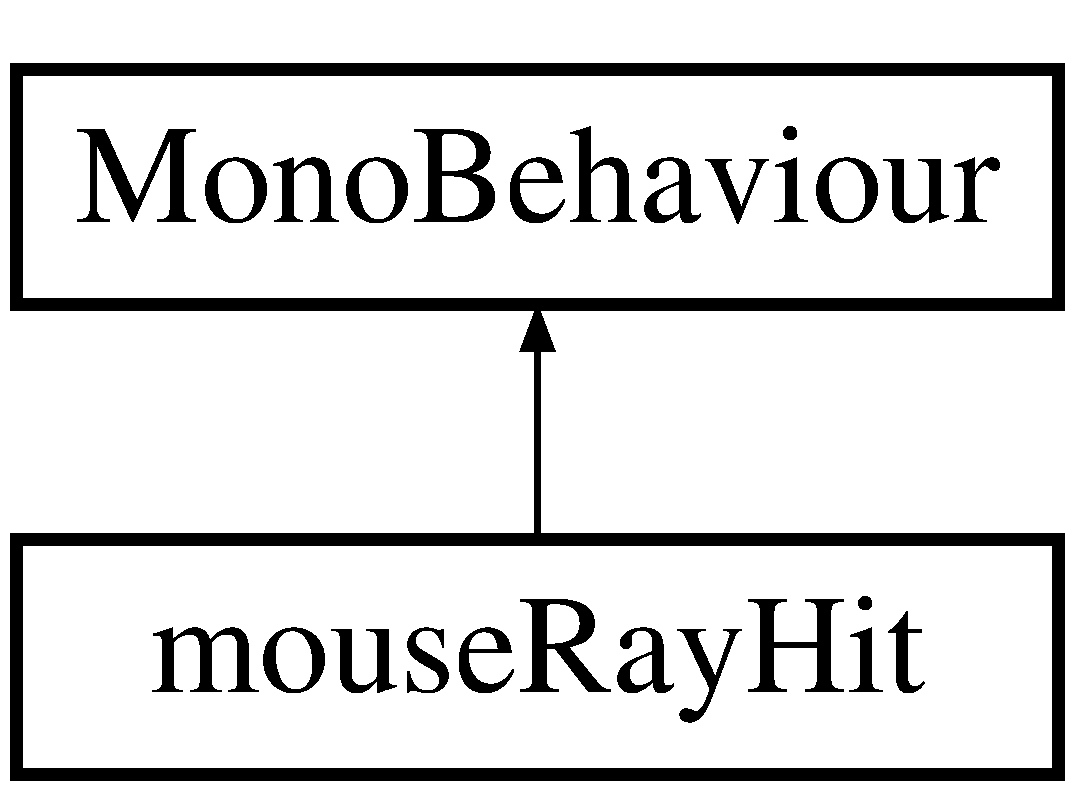
\includegraphics[height=2.000000cm]{classmouse_ray_hit}
\end{center}
\end{figure}


The documentation for this class was generated from the following file\+:\begin{DoxyCompactItemize}
\item 
Assets/\+\_\+\+Scripts/mouse\+Ray\+Hit.\+cs\end{DoxyCompactItemize}

\hypertarget{classmovement}{}\section{movement Class Reference}
\label{classmovement}\index{movement@{movement}}
Inheritance diagram for movement\+:\begin{figure}[H]
\begin{center}
\leavevmode
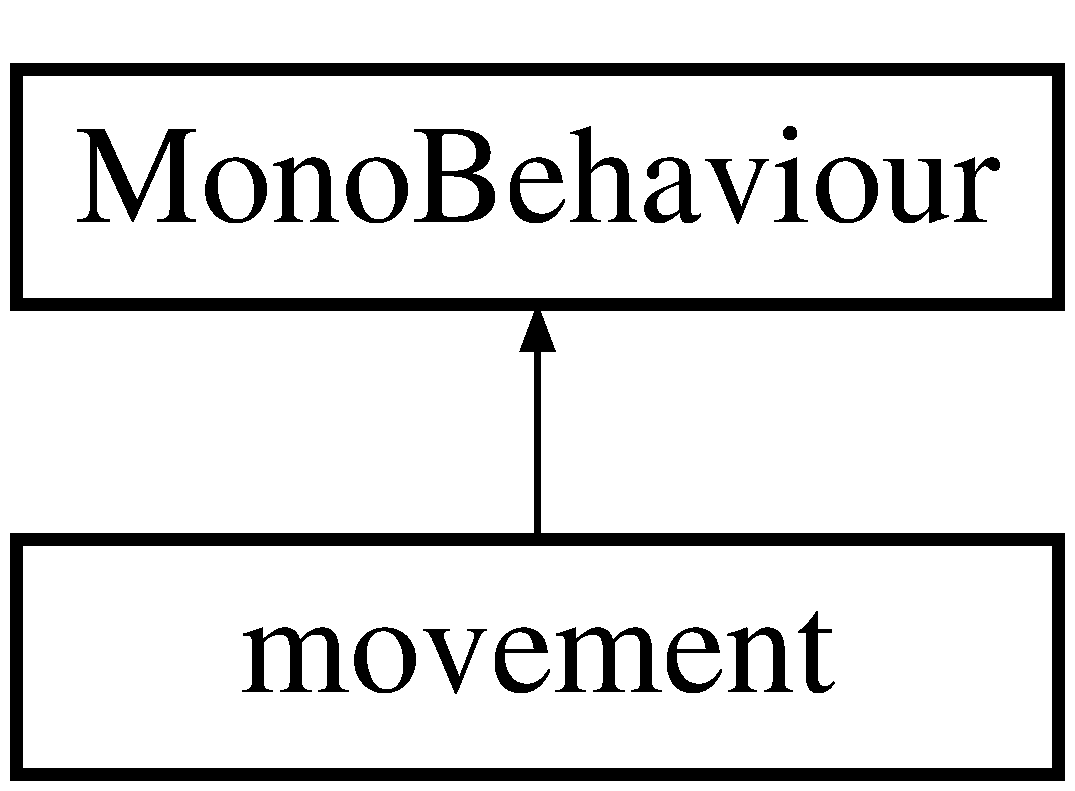
\includegraphics[height=2.000000cm]{classmovement}
\end{center}
\end{figure}
\subsection*{Public Attributes}
\begin{DoxyCompactItemize}
\item 
\hypertarget{classmovement_a853bd1ba34a86d555ebfad0e4bb2f4dd}{}Transform {\bfseries destination}\label{classmovement_a853bd1ba34a86d555ebfad0e4bb2f4dd}

\end{DoxyCompactItemize}


The documentation for this class was generated from the following file\+:\begin{DoxyCompactItemize}
\item 
Assets/\+\_\+\+Scripts/movement.\+cs\end{DoxyCompactItemize}

\hypertarget{classrandom_instance}{}\section{random\+Instance Class Reference}
\label{classrandom_instance}\index{random\+Instance@{random\+Instance}}
Inheritance diagram for random\+Instance\+:\begin{figure}[H]
\begin{center}
\leavevmode
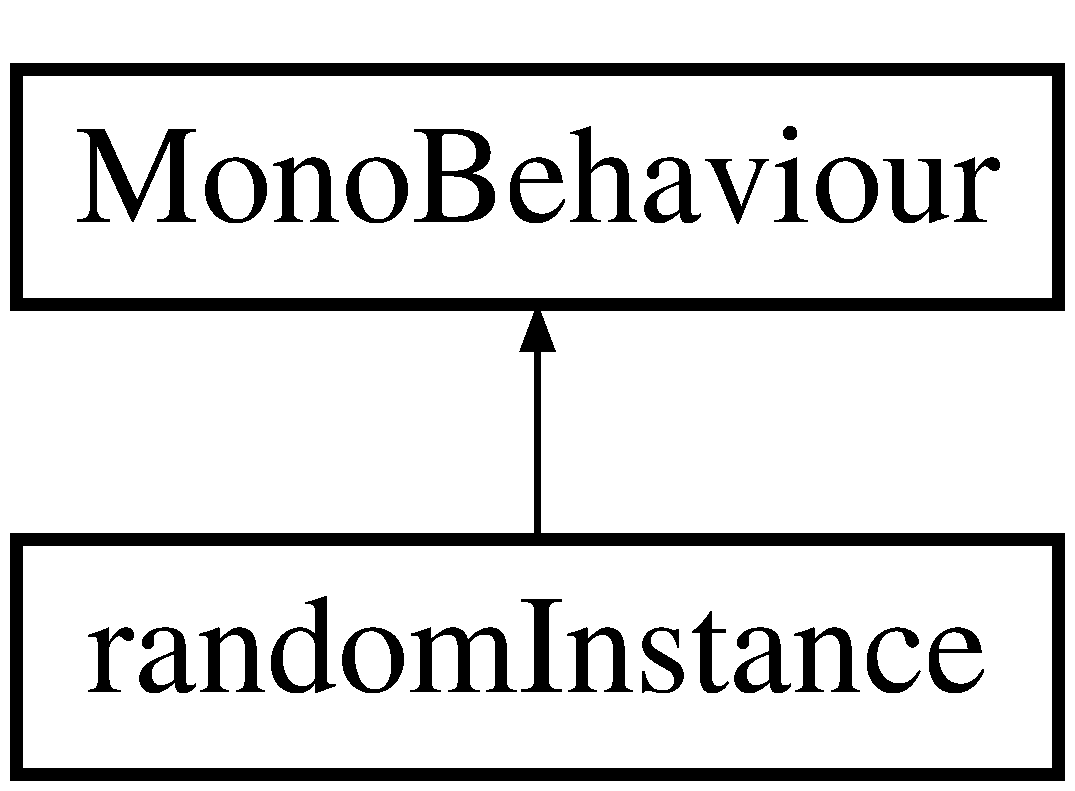
\includegraphics[height=2.000000cm]{classrandom_instance}
\end{center}
\end{figure}
\subsection*{Public Attributes}
\begin{DoxyCompactItemize}
\item 
Game\+Object \hyperlink{classrandom_instance_ad4bc8c2a580c04743c7ffb1aef90eaa6}{marker}
\item 
Game\+Object \hyperlink{classrandom_instance_aa1cf4fffeff6817cf74a11edb50dab5f}{garage}
\item 
Vector3 \hyperlink{classrandom_instance_a33ee46bc94d972337d4b332f1473ed1b}{map\+Limits}
\end{DoxyCompactItemize}
\subsection*{Static Public Attributes}
\begin{DoxyCompactItemize}
\item 
\hypertarget{classrandom_instance_a0e86ebd9e4ae8c213298a67742ba29ef}{}static int {\bfseries unit\+Send} = 0\label{classrandom_instance_a0e86ebd9e4ae8c213298a67742ba29ef}

\item 
\hypertarget{classrandom_instance_a44cf85cfa5c859825c4c2a8a466a2dda}{}static int {\bfseries unit\+Count} = 10\label{classrandom_instance_a44cf85cfa5c859825c4c2a8a466a2dda}

\item 
\hypertarget{classrandom_instance_acfb2f0ab3a2186cc8e00fb49764a062e}{}static int {\bfseries crime\+Count}\label{classrandom_instance_acfb2f0ab3a2186cc8e00fb49764a062e}

\item 
\hypertarget{classrandom_instance_a8c5866e85f8e8ebac681a2b30c28778d}{}static int {\bfseries money} = 1000\label{classrandom_instance_a8c5866e85f8e8ebac681a2b30c28778d}

\item 
\hypertarget{classrandom_instance_a629e99da5bdf553a859a127a62cbe3d9}{}static int {\bfseries unit\+Wage} = 100\label{classrandom_instance_a629e99da5bdf553a859a127a62cbe3d9}

\item 
\hypertarget{classrandom_instance_ad0bd7b1f32448fead10ff7dab284fadb}{}static int {\bfseries day} = 30\label{classrandom_instance_ad0bd7b1f32448fead10ff7dab284fadb}

\item 
\hypertarget{classrandom_instance_a5d7d3e6d79479d6f06c6a8eb52d8d078}{}static int {\bfseries month} = 12\label{classrandom_instance_a5d7d3e6d79479d6f06c6a8eb52d8d078}

\item 
\hypertarget{classrandom_instance_aa2c4ad17b10e4be3eddaeb02d43db34f}{}static int {\bfseries year} = 2000\label{classrandom_instance_aa2c4ad17b10e4be3eddaeb02d43db34f}

\item 
\hypertarget{classrandom_instance_af83397aaf6ed43e884247bb4d490bbc9}{}static int {\bfseries time\+Hour} = 23\label{classrandom_instance_af83397aaf6ed43e884247bb4d490bbc9}

\item 
\hypertarget{classrandom_instance_ab0fd3847ec9c0982e51074153d8b9722}{}static int {\bfseries unit\+Satisfaction} = 500\label{classrandom_instance_ab0fd3847ec9c0982e51074153d8b9722}

\item 
\hypertarget{classrandom_instance_a36cdfc1a24517e8fc3839358da61f01f}{}static float {\bfseries time\+Min} = 50\label{classrandom_instance_a36cdfc1a24517e8fc3839358da61f01f}

\end{DoxyCompactItemize}


\subsection{Member Data Documentation}
\hypertarget{classrandom_instance_aa1cf4fffeff6817cf74a11edb50dab5f}{}\index{random\+Instance@{random\+Instance}!garage@{garage}}
\index{garage@{garage}!random\+Instance@{random\+Instance}}
\subsubsection[{garage}]{\setlength{\rightskip}{0pt plus 5cm}Game\+Object random\+Instance.\+garage}\label{classrandom_instance_aa1cf4fffeff6817cf74a11edb50dab5f}
return point for the cars \hypertarget{classrandom_instance_a33ee46bc94d972337d4b332f1473ed1b}{}\index{random\+Instance@{random\+Instance}!map\+Limits@{map\+Limits}}
\index{map\+Limits@{map\+Limits}!random\+Instance@{random\+Instance}}
\subsubsection[{map\+Limits}]{\setlength{\rightskip}{0pt plus 5cm}Vector3 random\+Instance.\+map\+Limits}\label{classrandom_instance_a33ee46bc94d972337d4b332f1473ed1b}
limits for the camera \hypertarget{classrandom_instance_ad4bc8c2a580c04743c7ffb1aef90eaa6}{}\index{random\+Instance@{random\+Instance}!marker@{marker}}
\index{marker@{marker}!random\+Instance@{random\+Instance}}
\subsubsection[{marker}]{\setlength{\rightskip}{0pt plus 5cm}Game\+Object random\+Instance.\+marker}\label{classrandom_instance_ad4bc8c2a580c04743c7ffb1aef90eaa6}
target for the police cars 

The documentation for this class was generated from the following file\+:\begin{DoxyCompactItemize}
\item 
Assets/\+\_\+\+Scripts/random\+Instance.\+cs\end{DoxyCompactItemize}

\hypertarget{classstore_cars}{}\section{store\+Cars Class Reference}
\label{classstore_cars}\index{store\+Cars@{store\+Cars}}
Inheritance diagram for store\+Cars\+:\begin{figure}[H]
\begin{center}
\leavevmode
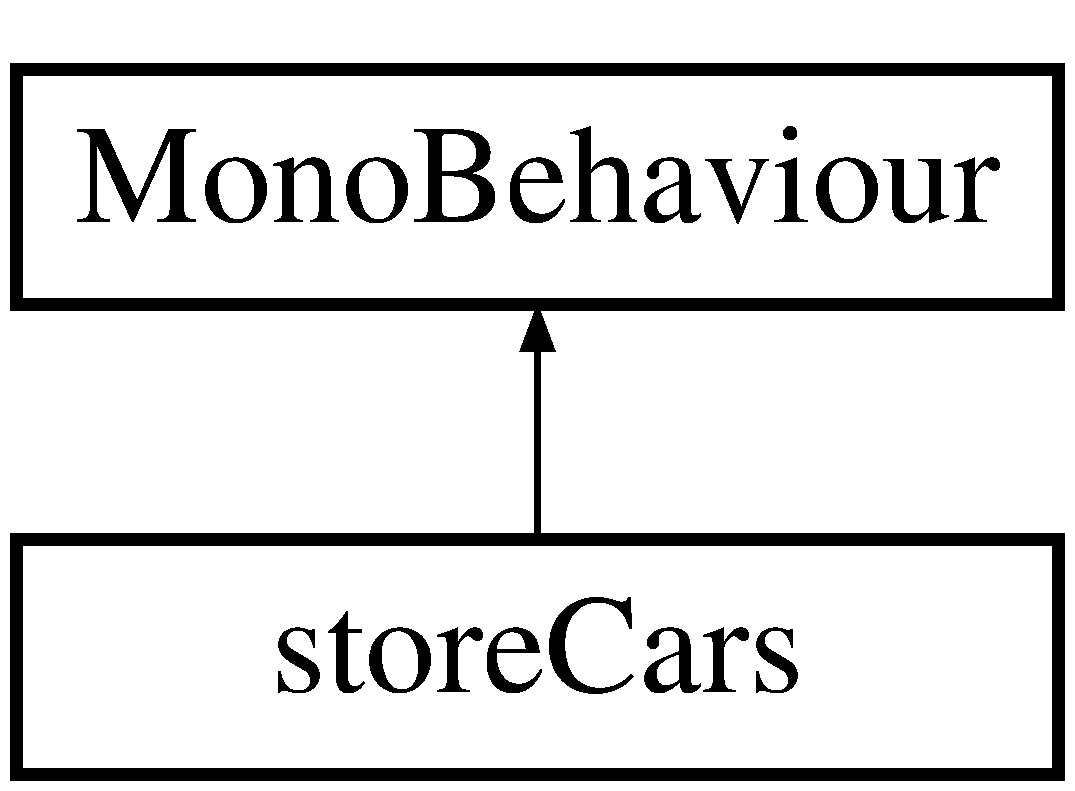
\includegraphics[height=2.000000cm]{classstore_cars}
\end{center}
\end{figure}


The documentation for this class was generated from the following file\+:\begin{DoxyCompactItemize}
\item 
Assets/\+\_\+\+Scripts/store\+Cars.\+cs\end{DoxyCompactItemize}

%--- End generated contents ---

% Index
\backmatter
\newpage
\phantomsection
\clearemptydoublepage
\addcontentsline{toc}{chapter}{Index}
\printindex

\end{document}
